\documentclass[fontsize=11pt]{article}
\usepackage{amsmath}
\usepackage[utf8]{inputenc}
\usepackage[margin=0.75in]{geometry}
\usepackage{csquotes}
\usepackage{hyperref}
\usepackage{amsmath}
\usepackage{tikz}
\usepackage[ruled,vlined,linesnumbered,noresetcount]{algorithm2e}
\usepackage{pythonhighlight}
\hypersetup{
    colorlinks=true,
    urlcolor=blue
    }


\title{CSC111 Project 2 Report Dishcovery}
\author{Alan Su, Yiping Chen, Defne Eris, Lily Phan}
\date{\today}

\begin{document}

\maketitle

\section{Introduction}
\par There is a demand for personalization in life. You want to feel special like something was "made for you". You have literal "for you" pages on social media which are curated to your interests, and you are recommended movies based on your past favourites but what about in the kitchen? \newline

\par As university students, we all know that making meals can be a struggle. Sometimes we do not know what to make or how to make it--and it is in times like these that we rely on recipes. When cooking, there's no one-size-fits-all recipe, everyone has their preferences and some recipes just don't cut it. Each person has their unique flavour preferences, dietary restrictions, and different levels of culinary literacy. It is hard to find a recipe that checks all the right boxes and even the perfect recipe might not be perfect for you. Sometimes, you aren't looking for any specific recipe and you just want to be pleasantly surprised with a recipe.  Cooking isn’t easy when you can’t find the right recipe. And with what recipes you like, you are stuck in a cycle where the most you can do is repeat the same recipes over and over you are bound to get bored and start looking elsewhere for variety, but as we have established recipe testing wastes a lot of time.\newline

\par We all know the feeling when we don't know what to eat but are picky about all the options. We just want someone else to figure out the perfect dish for us that we don't even know. Dish-covery is valuable in its personalization, it is the answer to the question: \textbf{How can we recommend recipes that are tailored to the user's specific needs?}  Dish-covery uses a recipe of your choice and offers new recipes based on a recipe we know you already like so that the recommended recipe won't disappoint. Dish-covery gets rid of the recipe search time so that you will always have a recipe that isn’t just suitable by others’ standards but your own. A recipe is more than just the end result, but its enjoy-ability can also be measured through the cooking process as well as how the instructions are presented. Dish-covery is able to gauge the recipes' similarity with others considering their performance among other customers and successfully generate a list of similar recipes. Using Dish-covery, the next time you try a new recipe you won't be "testing" it because you will know it is just right. \newline

\section{Data Sets}
Our data is collected from \href{https://cseweb.ucsd.edu/~jmcauley/datasets.html#foodcom}{Food.com's Recipe and Review Data}. More specifically, the \href{https://www.kaggle.com/datasets/shuyangli94/food-com-recipes-and-user-interactions/data?select=RAW_recipes.csv}{\texttt{RAW\_recipes.csv}} and the \href{https://www.kaggle.com/datasets/shuyangli94/food-com-recipes-and-user-interactions/data?select=RAW_interactions.csv}{\texttt{RAW\_interactions.csv}} files. The dataset is structured into two main components: the recipes and the reviews. Here is a (shortened) sample recipe for Beer Mac \& Cheese Soup:
\begin{center}\texttt{\begin{tabular}{ r l }
 name: & beer mac n cheese soup \\ 
 id: & 499490 \\  
 minutes: & 45 \\
 contributor\_id: & 560491 \\
submitted: & 2013-04-27 \\
tags: & 60-minutes-or-less
                    time-to-make
                    preparation \\
nutrition: & 678.8
                    70.0
                    20.0
                    46.0
                    61.0
                    134.0
                    11.0 \\
n\_steps: & 7 \\
steps: & cook the bacon in a pan over medium heat and set aside on... \\
ingredients: & bacon onion carrots celery... \\
n\_ingredients: & 17 \\
\end{tabular}}\end{center}
The recipe metadata is formatted as a csv file, where the columns correspond to the recipe's name, id, minutes (to prepare and cook), contributor's id, date submitted, tags, nutrition, number of steps, (description of the) steps, ingredients, and number of ingredients. The name is provided as a string, while the steps, ingredients, and tags are provided as a list of strings. The recipe's id, minutes, contributor's id, number of steps, and number of ingredients are provided as integers, while the nutrition is provided as a list of floats. The date is provided as a string in the form YYYY-MM-DD. However, the contributor's id, number of steps, and number of ingredients columns are not stored when the dataset is loaded to save on computation time and memory. \\
Here is a corresponding sample review for the recipe shown above:
\begin{center}\texttt{\begin{tabular}{ r l }
user\_id: & 8937 \\ 
recipe\_id: & 44394 \\
date: & 2002-12-01 \\
rating: & 4 \\
review: & This worked very well and is EASY...
\end{tabular}}\end{center}
The review metadata is also formatted as a csv file, where the columns correspond to the reviewing user's id as an integer, the id of the recipe being reviewed as an integer, the date reviewed as a similarly formatted string in the form YYYY-MM-DD, the rating as an integer from 1-5 inclusive, and a textual description of the review as a string. 

Only a subset of the vertices were used in the default implementation that loads the weighted recipe graph from the datasets, using the \texttt{recipes\_small.csv} and \texttt{interactions\_small.csv} files instead of the \texttt{recipes.csv} and \texttt{interactions.csv} files (renamed versions of the \texttt{RAW\_recipes.csv} and \texttt{RAW\_interactions.csv}, respectively). There are 500 of these vertices, as opposed to the $\approx$ 500,000 vertices (defined for each unique recipe and user id) in the original dataset. These vertices were chosen using the \texttt{densest\_subgraph} method of the \texttt{WeightedGraph} class, an implementation of the Charikar's greedy algorithm (See section 3.2 p.2) to determine the subgraph of with the highest amount of edges, given an amount of vertices (in this case, 500). The smaller versions of the original datasets only include rows which have vertices and edges which are contained within the computed 500 vertices. 

\section{Computational Overview}
\subsection{Notation}
Let $G = (V, E)$ be a bipartite graph consisting of two disjoint vertex sets $A = \{a_1, a_2, a_3, ..., a_{|A|}\}$ and $B = \{b_1, b_2, b_3, ..., b_{|B|}\}$ such that $V = A \cup B$ with edges $(a_i, b_j, w(a_i, b_j))$ in $E$ denoting a vertex $a_i$ in $A$ is connected to $b_j$ in $B$ with weight $w(a_i, b_j)$. For some vertex $v$, we denote $N(v)$ to be the set of the neighbours of $v$, and $d(v)$ be the degree of the vertices $v$. For some subgraph $G'=(V', E')$, we denote the density as $D(G') = \frac{\lvert E' \rvert}{\lvert V' \rvert}$. 

\subsection{Densest $k$ Subgraph}
Many of the algorithmns involved in calculating the similarity between two nodes are computational intensive, with, for example, Simrank being $\mathcal{O}(n^4)$, where $n$ is the number of vertices in a graph. In addition, the \texttt{nltk} sentiment analyzer is also computationally intensive, in particular because of the large amount of edges provided by the dataset. Thus, finding a subset of these vertices that contain the most amount of information and interactions between the user's reviews and the most popular recipes is necessary to answer queries searching for similar recipes in a reasonable amount of time, albeit with less overall variety in the recipes available. A graph is necessary for this computation as the measure of "information," denoted as the density function, $D$, uses the edges of the graph, which represents the reviews by the users. In other words, to reduce the graph's size down to a reasonable degree while keeping the most amount of information, a select subset of vertices representing the recipes and users should be selected such that it maximizes the number of reviews between vertices in this subset. 

The problem description involves finding the subgraph $G'$ with exactly $k$ vertices such that its density, $D(G')$, is maximized. Charikar (Varungohil, 2019) developed a simple greedy algorithm that calculates the optimal solution. The algorithm begins with a graph $G$ and repeatedly iterates over it until $\lvert V \rvert = k$. Each iteration, the algorithm identifies the vertex with the lowest degree, $v_{\text{min}}$, removes all edges connected to the vertex, and then removes $v_{\text{min}}$ from the graph of $G$. The resulting graph should contain vertices maximizing $D(S)$, for some subset $S \subseteq V$ where $\lvert S \rvert = k$.

\begin{algorithm}[H]
    \setcounter{AlgoLine}{0}
    \caption{\textsc{densest\_subgraph} Charikar's Greedy Algorithm for Densest $k$ Subgraph}
    \SetKwInOut{Input}{Input}
    \SetKwInOut{Output}{Output}
    \Input{Undirected graph $G$, subgraph size $k$.}
    \While{$\lvert V \rvert > k$}{
        $v_{\text{min}}$; $n_{v_{\text{min}}} \gets \infty$\;
        \For{$v_i \in V$}{
            \If{$\lvert N(v_i) \rvert < n_{v_{\text{min}}}$}{
                $v_{\text{min}} \gets v_i$\;
                $n_{v_{\text{min}}} \gets \lvert N(v_i) \rvert$\;
            }
        }
        \For{$v_i \in N(v_{\text{min}})$}{
            $N(v_i) \gets N(v_i) \setminus \{v_{\text{min}}\}$\;
        }
        $V \gets V \setminus \{v_{\text{min}}\}$
    }
\end{algorithm}

Algorithm 1 illustrates the pseudo-code for the \textsc{densest\_subgraph} method using Charikar's greedy approach, which iteratively removes the lowest degree vertex. To test this method, you can run the \texttt{graph.py} file in the Python console and find the subgraph of 50 vertices with the highest density out of the reduced 500 vertex graph:
\begin{python}
>>> graph = load_weighted_review_graph(file_paths={'interactions': 'data/interactions_small.csv', 'recipes': 'data/recipes_small.csv'}, load_precomputed=False)
>>> graph.densest_subgraph(subgraph_size=50, file_path='data/vertices_mini.txt')
\end{python}
Or alternatively, you may attempt to find the subgraph of 500 vertices with the highest density out of the original $\approx$ 500,000 vertex graph, which had a total runtime of around 3 hours. To save on computation time, the sentiment scores are not loaded.
\begin{python}
>>> graph = load_weighted_review_graph(file_paths={'interactions': 'data/interactions.csv', 'recipes': 'data/recipes.csv'}, load_precomputed=False, load_sentiment=False)
>>> graph.densest_subgraph(subgraph_size=500, file_path='data/new_vertices.txt')
\end{python}
After the subgraph's vertices are identified, they are stored in a file specified by the \texttt{file\_paths} argument. You can call the \texttt{generate\_subgraph\_dataset} with the new file path to create a new dataset with only the dense subgraph's vertices and edges, after which they can be loaded again, using the newly generated datasets.
\begin{python}
>>> graph.generate_subgraph_dataset(file_paths={'new_vertices': 'data/vertices_mini.txt', 'interactions': 'data/interactions_small.csv', 'recipes': 'data/recipes_small.csv', 'new_interactions': 'data/interactions_mini.csv', 'new_recipes': 'data/recipes_mini.csv'})
>>> graph = load_weighted_review_graph(file_paths={'interactions': 'data/interactions_mini.csv', 'recipes': 'data/recipes_mini.csv'}, load_precomputed=False)
\end{python}

\subsection{Jaccard Similarity}
One of the most common measures of similarity between two vectors or vertices in a graph is the Jaccard similarity. For two vertices $a \in A$ and $b \in B$, the Jaccard similarity, $s_{\text{Jaccard}}$, on a weighted graph follows the formula:
\[
s_{\text{Jaccard}}(a, b) = \frac{\sum_{v \in N(a) \cup N(b)}\min(w(a, v), w(b, v))}{\sum_{v \in N(a) \cup N(b)}\max(w(a, v), w(b, v))}
\]
Calculated by dividing the sum of the minimum weights of the edges connected to either vertex $a$ or $b$, by the maximum sum, the Jaccard similarity is used on this dataset as its representation as a graph is bipartite. The vertices in the graph may be separated into two disjoint sets, $A$, and $B$, representing the users and the recipes, where the edges, which signify a review, only connect a user with the corresponding recipe they reviewed. Note that for some edge connecting a user, $u$, with a recipe, $v$ with their review, if the user never reviewed the recipe, then $w(u, v) = 0$. 

While this similarity metric is not computationally intensive, implemented in the \texttt{graph.py} using the \pyth{jaccard_sim} method of the \pyth{_WeightedVertex} class and running in $\mathcal{O}(\lvert V \rvert)$ time, it only considers and uses vertices that are directly adjacent to $a$ or $b$ in its computation, which does makes it less ideal in datasets with less edges that are more sparsely connected. The resultant Jaccard similarity score is $0 \leq s_{\text{Jaccard}}(a, b) \leq 1$. Graphs, in particular, are necessary for this computation as the vertices the edges with their neighbours define how the score is calculated.

\subsection{Overlap Similarity}
Another useful metric for calculating the similarity between two vertices, $a \in A$ and $b \in B$, in a bipartite graph, is the Overlap Similarity. While similar to the Jaccard Similarity, it may perform better in specific situations, and is defined by the formula:
\[
s_{\text{Overlap}}(a, b) = \frac{\sum_{v \in N(a) \cup N(b)}\min(w(a, v), w(b, v))}{\min(\sum_{v \in N(a)}w(a, v), \sum_{v \in N(b)}w(b, v)))}
\]
The Overlap similarity metric is calculated, like the Jaccard similarity, by dividing the sum of the minimum weights of the edges connected to either vertex $a$ or $b$, instead being divided by the minimum total sum of the weights connected to $a$ or $b$. It shares many of the strengths and weaknesses of the Jaccard similarity metric, with a low computational overhead, running in $\mathcal{O}(\lvert V \rvert)$ time, but at the cost of only considering vertices directly adjacent to the two vertices that are passed into the function. It is implemented in using the \pyth{overlap_sim} method, and its result, $s_{\text{Overlap}}(a, b)$ falls between 0 and 1. Like the Jaccard similarity metric, it uses the crucial aspect of graphs, its edges, to calculate the similarity, which likely wouldn't be possible on other data types.

\subsection{Cosine Similarity}
The Cosine similarity metric is another common similarity metric used on either a pair of vectors or vertices of a graph. Unlike the Jaccard or Overlap similarity, it does not use the minimum, instead using the dot product and norm of two vectors, or two sets of weights, following the formula:
\[
s_{\text{Cosine}}(a, b) = \sum_{u \in N(a) \cup N(b)} \frac{w(a, u) \cdot w(b, u)}{\sqrt{\sum_{v \in N(a)}w(a, v)^2}\sqrt{\sum_{v \in N(b)}w(b, v)^2}}
\]
Calculated by dividing the dot product of the weights of the neighbouring vertices of $a$ or $b$ by the product of the norm of the neighbours of $a$ and $b$, the Cosine similarity metric is $\mathcal{O}(\lvert V \rvert)$ although similarly only considers vertices directly adjacent to either $a$ or $b$. Implemented in the \pyth{cosine_sim} method, the similarity metric outputs a number between 0 and 1, using the edges of a graph which are necessary to calculate the Cosine similarity. 

\subsection{Tanimoto Similarity}
The Tanimoto similarity is often used in many scientific fields as a measure of the closeness or as a basis of comparison. It follows the formula:
\[
s_{\text{Tanimoto}}(a, b) = \frac{\sum_{u \in N(a) \cup N(b)} w(a, u) \cdot w(b, u)}{\sum_{v \in N(a)}w(a, v)^2 + \sum_{v \in N(b)}w(b, v)^2 - \sum_{u \in N(a) \cup N(b)} w(a, u) \cdot w(b, u)}
\]
It shares around the same computation time, being $\mathcal{O}(\lvert V \rvert)$, and its results fall between 0 and 1. The similarity metric is implemented in the \pyth{tanimoto_sim} method, and necessarily uses the graph weights to determine the final metric. 

\subsection{Simrank}
Many of the previous metrics shown suffer from finding the similarity between vertices which do not share direct neighbours, even when they may have many similar aspects. As a solution to this, Simrank is an iterative algorithm which follows the key idea that "two objects are considered similar if they are referenced by similar objects." Proposed by Jeh and Widow (\color{red}TODO: cite \href{https://www.cse.cuhk.edu.hk/~cslui/CMSC5734/simrank.pdf}{this}\color{black}) in a 2002 paper, 

The algorithm iteratively calculates the Simrank similarity metric, $S$, by first assigning the starting similarity, $S_1$ between two nodes, $a \in V$ and $b \in V$ to defined as:
\[S_0(a, b) = \begin{cases}
    1 & \text{if } a = b \\
    0 & \text{if } a \neq b
\end{cases}\]
Then, it iteratively calculates the Simrank similarity metric following the equation, where C is the decay factor, typically set to a value of $C=0.9$:
\[
S_{k+1}(a, b) = \frac{C}{\lvert N(a) \rvert \lvert N(b) \rvert} \sum^{\lvert N(a) \rvert}_{u \in N(a)} \sum^{\lvert N(b) \rvert}_{v \in N(b)} S_k(a, b) \cdot w(a, u) \cdot w(b, v)
\]
This continues until $S_k(a, b)$ converges as $k \to \infty$, to get $S(a, b) = \lim_{k \to \infty}S_k(a, b)$. In practice, we use an error threshold to determine the maximum difference our computed result can be from the final. 

\begin{algorithm}[H]
    \setcounter{AlgoLine}{0}
    \caption{\textsc{CalculateSimrank}}
    \SetKwInOut{Input}{Input}
    \SetKwInOut{Output}{Output}
    \Input{Graph $G$, Simrank similarities $S_k$, vertices $a, b \in V$, decay factor $C$}
    \Output{$S_{k+1}(a, b)$}
    \lIf{$a = b$}{\Return 1}
    \lIf{$\lvert N(a) \rvert = 0 \lor \lvert N(b) \rvert = 0$}{\Return 0}
    $n_{\text{sum}} \gets 0$\;
    \For{$u \in N(a)$}{
        \For{$v \in N(b)$}{
            $n_{\text{sum}} \gets n_{\text{sum}} + S_k(a, b) \cdot w(a, u) \cdot w(b, v)$\;
        }
    }
    \Return $\frac{C}{\lvert N(a) \rvert \lvert N(b) \rvert} n_{\text{sum}}$\;
\end{algorithm}

Algorithm 2 is the pseudo-code of how one iteration of Simrank may be calculated, using the previous formula and the decay factor to compute the new Simrank values. For each iteration, the Simrank algorithm takes follows $\mathcal{O}(\lvert N(a) \rvert \lvert N(b) \rvert)$ time, and returns a value $0 \leq S_{k+1} \leq 1$. 

\begin{algorithm}[H]
    \setcounter{AlgoLine}{0}
    \caption{\textsc{Simrank}}
    \SetKwInOut{Input}{Input}
    \SetKwInOut{Output}{Output}
    \Input{Graph $G$, starting Simrank similarities $S_0$, decay factor $C$, error threshold $\epsilon_f$}
    \Output{$S(a, b) \mid a \in V, b \in V$}
    $\epsilon \gets \infty$\;
    $k \gets 0$\;
    $S_k \gets S_0$\;
    \While{$\epsilon > \epsilon_f$}{
        $S_{k+1}$\;
        $\epsilon \gets 0$\;
        \For{$a \in V$}{
            \For{$b \in V$}{
                   $S_{k+1}(a, b) \gets \textsc{CalculateSimrank}(G, S_k, a, b, C)$\;
                   $\epsilon \gets \epsilon + \lvert S_{k+1} - S_{k} \rvert$
            }
        }
        $k \gets k+1$\;
        $S_k \gets S_{k+1}$\;
        $\epsilon \gets \frac{\epsilon}{\lvert V \rvert}$\;
    }
    \Return $S_k$\;
\end{algorithm}

Algorithm 3 illustrates the pseudo-code for an iterative computation to determine the Simrank similarity metric between each pair of vertices in the graph of $G$. It takes advantage of the function in Algorithm 2, \textsc{CalculateSimrank}, to calculate the similarity scores between a specific pair of vertices. Including the \textsc{CalculateSimrank} function, Algorithm 3 is $\mathcal{O}(\lvert V \rvert^4)$, which makes is computationally intensive for graphs with many vertices. However, unlike the Jaccard, Overlap, Cosine, and Tanimoto similarty measures, the similarity measure takes vertices other than those directly adjacent to the two vertices passed into the function to determine the final similarity, at the cost of computational time. As a result, the Simrank similarity metric for each pair of vertices is should be pre-computed to answer the queries the users have in real time. To test this method, run the \texttt{graph.py} file in the Python console, without loading the already pre-computed values, and then directly pre-compute for yourself the Simrank similarity values.

\begin{python}
>>> graph = load_weighted_review_graph(load_precomputed=False)
>>> graph.simrank(pplus=False, file_path='data/new_simrank.json')
\end{python}

While this by default loads the reduced 500 vertex graph instead of the $\approx$ 500,000 vertex graph, it is expected the Simrank algorithm still may take around 5-10 minutes to run, due to the high time complexity of the algorithm. After it completes, the graph can be loaded again with the new pre-computed Simrank similarity values and you can attempt to directly recommend some recipes using the newly calculated metric.

\begin{python}
>>> graph = load_weighted_review_graph(file_paths={'simrank': 'data/new_simrank.json'}, load_precomputed=True)
>>> graph.recommend_recipes('moms pizza spaghetti', limit=3, score_type='simrank')
\end{python}

As Simrank relies on the central idea of how similar vertices are connected by similar vertices, thus it is necessary to use a graph to both compute and represent the values for the similarties using Simrank between the vertices in the graph. Graphs are central as they are an important element in the Simrank formula and computation, as their edges define how similar vertices are connected by similar vertices. 

\subsection{Simrank++}
One issue with Simrank is that it does not account for the number of common neighbours that are shared between the two nodes that have their similarity being calculated. Normally, the more common neighbours two vertices share, then the higher the similarity score they should have. However, in reality, the Simrank similarity score is often lower for vertices which share many of the same neighbours when compared to vertices which only have, for example, one shared neighbour. 

\begin{center}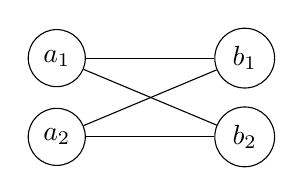
\begin{tikzpicture}[main/.style = {draw, circle}, node distance=1cm] 
\node[main] (1) {$a_1$}; 
\node[main] (2) [below of=1] {$a_2$};
\node[main] (3) [right=2cm] {$b_1$}; 
\node[main] (4) [below of=3] {$b_2$}; 
\draw (1) -- (3);
\draw (1) -- (4);
\draw (2) -- (3);
\draw (2) -- (4);
\end{tikzpicture}\\
Figure 1\\[1cm]
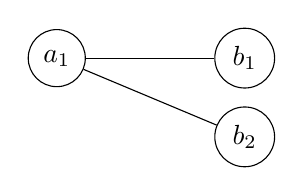
\begin{tikzpicture}[main/.style = {draw, circle}, node distance=1cm] 
\node[main] (1) {$a_1$}; 
\node[main] (2) [right=2cm] {$b_1$};
\node[main] (3) [below of=2] {$b_2$}; 
\draw (1) -- (2);
\draw (1) -- (3);
\end{tikzpicture}\\
Figure 2
\end{center}

For example, while one might assume that the vertices $a_1$ and $a_2$ have a higher similarity score in Figure 1, as opposed to the vertices $a_1$ and $a_2$ in Figure 2 (\color{red}There is no $a_2$ in Figure 2\color{black}). However, in reality, the Simrank similarity score for the first figure converges at approximately $\approx 0.67$, while the Simrank similarity score for the second pair of vertices, in Figure 2, is 0.8. 

Simrank++, developed by Antonellis, Garcia-Molina, and Chang in a 2007 paper (\color{red}TODO: cite \href{https://arxiv.org/pdf/0712.0499.pdf}{this} lmao\color{black}), provides a solution to this problem. Simrank++, an alternate version of the Simrank similarity metric, attempts to resolve this issue by introducing a new factor called evidence, which increases the similarity score based on the number of common neighbours between the vertices being evaluated. It follows the formula:

\[
S_{k+1}(a, b) = \left(\sum_{i=1}^{\lvert N(a) \cap N(b) \rvert}\frac{1}{2^i}\right) \cdot \frac{C}{\lvert N(a) \rvert \lvert N(b) \rvert} \sum^{\lvert N(a) \rvert}_{u \in N(a)} \sum^{\lvert N(b) \rvert}_{v \in N(b)} S_k(a, b) \cdot w(a, u) \cdot w(b, v)
\]

With this new formula, the Simrank++ evaluates to be around $\approx 0.50$ between the vertices $a_1$ and $a_2$ in Figure 1, while it evaluates to 0.4 for the vertices in Figure 2. 

\begin{algorithm}[H]
    \setcounter{AlgoLine}{0}
    \caption{\textsc{CalculateSimrank} for Simrank++}
    \SetKwInOut{Input}{Input}
    \SetKwInOut{Output}{Output}
    \Input{Graph $G$, Simrank similarities $S_k$, vertices $a, b \in V$, decay factor $C$}
    \Output{$S_{k+1}(a, b)$}
    \lIf{$a = b$}{\Return 1}
    \lIf{$\lvert N(a) \rvert = 0 \lor \lvert N(b) \rvert = 0$}{\Return 0}
    $n_{\text{sum}} \gets 0$\;
    \For{$u \in N(a)$}{
        \For{$v \in N(b)$}{
            $n_{\text{sum}} \gets n_{\text{sum}} + S_k(a, b) \cdot w(a, u) \cdot w(b, v)$\;
        }
    }
    $t \gets 0$\;
    \For{$i \gets 1$ to $\lvert N(a) \cap N(b) \rvert$}{
        $t \gets t + \frac{1}{2^i}$\;
    }
    \Return $t \cdot \frac{C}{\lvert N(a) \rvert \lvert N(b) \rvert} n_{\text{sum}}$\;
\end{algorithm}

Above, in Algorithm 4, is the pseudo-code for the \textsc{CalcualteSimrank} algorithm for two nodes $a$ and $b$, specifically using the Simrank++ formula instead of the Simrank one. The \textsc{Simrank} iteration algorithm for Simrank++ until convergence would be the same as the Simrank algorithm, except using Algorithm 4 instead. The Simrank++ method can be similarly tested compared to the Simrank, except \pyth{pplus} should be set to \pyth{True} in the Simrank iteration function after \texttt{graph.py} is run in the Python console.

\begin{python}
>>> graph = load_weighted_review_graph(load_precomputed=False)
>>> graph.simrank(pplus=True, file_path='data/new_simrank_pplus.json')
>>> graph = load_weighted_review_graph(file_paths={'simrank_pplus': 'data/new_simrank_pplus.json'}, load_precomputed=True)
>>> graph.recommend_recipes('moms pizza spaghetti', limit=3, score_type='simrank_pplus')
\end{python}

\subsection{Personalized Pagerank}
Pagerank is an algorithm commonly used to sort webpages based on their relevance to a specific search query. In particular, Google used it to order their webpages based on the quality and quantity of links referencing each other. First introduced in a paper in 1998, authors Brin and Page developed Pagerank (University of Pennsylvania, 1998) as a method to order relevant vertices in a graph. 

The Pagerank score of a vertex is based on the number of important nodes that reference, or are linked to it. In this case, it means that there is a review between an important user and a recipe or an important recipe and a user. In other words, many higher-scoring neighbours will result in a higher Pagerank similarity score than a vertex with lower-scoring neighbours. It can be thought of as a random walker, which begins on a specific vertex and on each iteration, travels to a random neighbouring vertex each iteration (depending on the weights, with a higher probability to travel to vertices with a stronger edge weight to the random walker's vertex). In addition, there is a random chance, called the damping factor, that instead of travelling to a neighbour, the walker is teleported to a random vertex on the graph. This is implemented to prevent dead ends in directed graphs where the walker gets stuck for the rest of the iteration. Then at the end, the number of times the walker visited each vertex is calculated, and divided by the total number of nodes, to arrive at a final Pagerank similarity score. 

In particular, the implemented version of the graph is a Personalized Pagerank algorithm, where instead of teleporting to a random vertex, there is a defined mapping of probabilities to each vertex and their associated probability of being teleported to. In this implementation, the personalization will always cause the vertex to teleport to the vertex in which the similarity is being calculated for. The Pagerank, $P(a, b)$ between two vertices $a$, and $b$, uses a random walk for each vertex in the graph to determine the similarities between every pair of vertices. 

\begin{algorithm}[H]
    \setcounter{AlgoLine}{0}
    \caption{\textsc{RandomWalk}}
    \SetKwInOut{Input}{Input}
    \SetKwInOut{Output}{Output}
    \Input{Graph $G$, starting vertex $a$, damping factor $\alpha$, error threshold $\epsilon_f$}
    \Output{$P(a, v), \forall v \in V$}
    $N_{\text{count}}(v) \gets 0, \forall v \in V$\;
    $u \gets a$\;
    $N_{\text{count}}(u) \gets 1$\;
    \For{$i \gets 1$ to $\lceil \frac{1}{\epsilon_f} \rceil$}{
        \eIf{$(100\cdot \alpha)$\% chance}{
            $u \gets $ vertex $b \in N(u)$, randomly selected based on $w(b, u)$\;
        }{
            $u \gets a$\;
        }
        $N_{\text{count}}(u) \gets N_{\text{count}}(u) + 1$\;
    }
    $t \gets 0$\;
    \lFor{$v \in V$}{$t \gets t + N_{\text{count}}(v)$}
    $P(a, v) = \frac{N_{\text{count}}(v)}{t}, \forall v \in V$\;
    \Return $P(a, v)$
\end{algorithm}

Above, Algorithm 5 illustrates the pseudo-code for the \textsc{RandomWalk} algorithm that is used to determine the PageRank similarity between node $a$, and every other node $v \in V$. The lower the error threshold, the more iterations of the random walk are performed. For each iteration, the Pagerank similarity algorithm takes $\mathcal{O}(\lceil \frac{1}{\epsilon_f} \rceil)$  time, assuming $\lceil \frac{1}{\epsilon_f} \rceil >> \lvert V \rvert$, and returns a value $0 \leq P(a, v) \leq 1$. 

\begin{algorithm}[H]
    \setcounter{AlgoLine}{0}
    \caption{\textsc{PageRank}}
    \SetKwInOut{Input}{Input}
    \SetKwInOut{Output}{Output}
    \Input{Graph $G$, damping factor $\alpha$, error threshold $\epsilon_f$}
    \Output{$P(a, b), \forall a \in V, \forall b \in V$}
    $P$\;
    \For{$a \in V$}{
        $P(a, b) \gets \textsc{RandomWalk}(G, a, \alpha, \epsilon_f), \forall b \in V$
    }
    \Return $P(a, b), \forall a \in V, \forall b \in V$
\end{algorithm}

Algorithm 6 illustrates the pseudo-code for the \textsc{Pagerank} algorithm, which calculates the Pagerank similarity score between every pair of vertices $a$ and $b$ in the graph of $G$. It uses the previously defined Algorithm 5, \textsc{RandomWalk}, using the damping factor and error threshold defined in the function. Taking $\mathcal{O}(\lceil \frac{1}{\epsilon_f} \rceil \cdot \lvert V \rvert)$ time, the algorithm is particularly computationally intensive when there is a low error threshold and a large amount of vertices in the graph. As a tradeoff, it can calculate the similarity scores accounting for vertices which do not share any directly adjacent vertexes, unlike some of the previously defined functions other than Simrank and Simrank++. Similarly, however, the similarity score values will need to be pre-computed for Pagerank in order to respond in real-time to queries made by the user without being computationally intensive. This method can be tested by running \texttt{graph.py} in the Python console, without loading the supplied pre-computed similarity score values, and instead, computing them yourself. 

\begin{python}
>>> graph = load_weighted_review_graph(load_precomputed=False)
>>> graph.pagerank(file_path='data/new_pagerank.json')
\end{python}

While by default, this function uses the smaller 500 vertex graph instead of the original one, the pre-computation for the Pagerank similarity scores may take around an hour. After it completes, the graph can then be loaded again by specifying the new pre-computed file path for the Pagerank similarity scores, and a recipe can be recommended.

\begin{python}
>>> graph = load_weighted_review_graph(file_paths={'pagerank': 'data/new_pagerank.json'}, load_precomputed=True)
>>> graph.recommend_recipes('moms pizza spaghetti', limit=3, score_type='pagerank')
\end{python}

Pagerank necessarily uses a graph as a crucial element in its calculation is its usage of the random walker, which is responsible for determining the similarity scores between vertices. However, without a graph and its edges, it would be difficult to determine the path of the random walker, thereby restricting the calculation of the Pagerank similarity scores. Thus, a graph is necessary to be utilized when calculating, especially with Pagerank, similarity scores. 

\subsection{Sentiment Analysis}
While calculating the similarity scores between each recipe, instead of only relying on user ratings, we wanted to give the user the option of taking the written reviews into account while calculating the similar recipes. Analyzing the written reviews can help differentiate between recipes that have similar ratings and give a more objective analysis of the similarities between each recipe. In order to perform a sentiment analysis the {\em nltk} (Natural Language Toolkit) library was used due to its large number of open sources and practical implementation. {\em NLTK} was created in 2001 by the Department of Computer and Information Science at the University of Pennsylvania with the goals of "Simplicity, Consistency, Practicality, Modularity" allowing the easy implementation of natural language processing. The library has been updated consistently and has been favored in research projects (Bird, Klein and Loper, 2019). While performing the sentiment analysis for each review, the \pyth{polarity_scores} method of the \pyth{SentimentIntensityAnalyzer} class was used in this algorithm. The \pyth{polarity_scores} method operates by returning a dictionary mapping each string with its associated negative, neutral, positive, and overall scores. The individual scores' values range from 0 to 1 inclusive and the overall score which is between -1 and 1 inclusive is calculated by combining the individual scores of the review. In our algorithm, since we only wanted to analyze the compound score of the review, only the overall scores for each review were used. The code below shows an example of passing in one of the reviews in our data set to the \pyth{polarity_scores} method.

\begin{python}
>>> from nltk.sentiment import SentimentIntensityAnalyzer
>>> sia = SentimentIntensityAnalyzer()
>>> sia.polarity_scores("Excellent!  The most simple, perfect, veggie dish.")
{'neg': 0.0, 'neu': 0.385, 'pos': 0.615, 'compound': 0.8389}
\end{python}

In the algorithm, the sentiment score analysis was done with the Sentiment Intensity Analyzer in {\em nltk} by reading the \texttt{interactions\_small.csv} file, calculating the overall sentiment scores of each review with the \pyth{polarity_scores} method, and returning a dictionary mapping review ids' with a list of tuples of the actual ratings and sentiment scores for each review. Then for each review, its sentiment score and actual rating were combined to give a new rating value ranging from 1 to 5 inclusive. And based on the user's input, if the user wanted to incorporate the sentiment scores of the reviews, these newly calculated ratings were used instead of the actual ratings for the similarity analysis.

\subsection{Visualizations with Tkinter}
When a user first opens our program, they are greeted by a starting screen which was drawn by us (the background was inspired by Cooking Mama's theme). The user presses the "Click Here to Begin" button to start the program, and is brought to a new frame where they can begin to enter in their criteria for their desired recipe. Note that the background was also drawn by us. They choose from a scrolling menu what their recipe is, and from dropdown bars they may also choose the type of recommendation system they want alongside if they want sentimental analysis to be used with it. The user may also enter in a numeric value for how many recommendations they want. Once the user confirms their choices, they may then click the "done" button which clears the screen and presents them a list of recipes our algorithms from before recommends, based on the information they inputted. Recipes will be presented from most highly recommended to not recommended. The recipe presented will include the most relevant information such as the name, description, steps, time needed, and ingredients for every recipe. If a user enters a very small number for the number of recipes they want, they're likely to only see the most highly recommended, but if they enter a large number like 500, it'll be easier to see which recipes were more recommended than others. Notably, while the algorithms themselves and the graph were not explicitly pictured in the visualization, the user is still able to see the results of it at the end with the recommendations, and interact with it as they can change the output of what recipes are recommended each time by inputting different values. \newline

We decided to go with the \pyth{Tkinter} library for several reasons. Note that all the code that uses this library is contained in the \pyth{gui.py} file. Part of the reason why we chose this library was because there was so many tutorials and documentations online, which made it easier for us to work with and understand how to use the library in a shorter amount of time. Additionally, Tkinter was very customizable, in that it was able to take in multiple forms of user input. For instance, we were able to use the \pyth{tk.OptionMenu()} method to create dropdown menus, and also use \pyth{tk.Entry()} method to allow the user to type in a number. This was useful as some forms of user input were more user friendly than others, such as using a scroll menu instead of an entry box for choosing the recipe. Another useful aspect of \pyth{Tkinter} is that it was very easy to understand how to arrange items on the frame. Throughout the program, \pyth{.place()} is used to organize the widgets on the screen and also scale them down or up to size. Moreover, Tkinter is great in that all the functionality we needed was essentially all in the Tkinter library already. We did not need to install additional files such as PIL to open images, which simplified our program.

\section{Instructions for use}
We sent our files via  https://send.utoronto.ca and shared it with the course email address, csc111-2023-01@cs.toronto.edu. It was sent by Alan. Start by opening up the \pyth{requirements.txt} file and installing all the libraries. Next, run the following code block in your console:
\begin{python}
import nltk
import ssl

try:
    _create_unverified_https_context = ssl._create_unverified_context
except AttributeError:
    pass
else:
    ssl._create_default_https_context = _create_unverified_https_context

nltk.download('vader_lexicon')
\end{python}
Following this, open the \pyth{main.py} file and run the main code block.
The first thing you should see is the starting screen.
\begin{figure}
    \centering
    \includegraphics[width=0.8\linewidth]{startscreen.png}
    \caption{The screen you should see when you first open the program}
    \label{fig:enter-label}
    \begin{flushleft} 
    After you press the click the "Click Here To Begin" button, you should see: \end{flushleft}
    
    \includegraphics[width=0.8\linewidth]{image.png}
    \caption{The screen you should see after clicking the "Click Here To Begin"}
    \label{fig:enter-label}
    \begin{flushleft} 
    This is the page where you will begin to choose your criteria. Select your recommendation system, sentiment, and number of recommendations first. Note that the recommendation system and sentiment values are dropdown menus, so you will need to press them to see all the options. Enter a number for the number of recommendations. \textbf{Choose your preferred recipe last.} This is because of how Tkinter works, in that it will not read in your selected choice from the scrolling menu unless your cursor was on that value before. Press confirm choice once you're happy, and press done to see the results. \end{flushleft}

    
\end{figure}

\begin{figure}
    \centering
    \includegraphics[width=0.8\linewidth]{image2.png}
    \caption{You should see a list of recommended recipes.}
    \label{fig:enter-label}
    \begin{flushleft}
        After you enter your criteria, something like the following page should appear. The recommended recipes will be displayed in order from most recommended to least, and you can scroll through to see all the recommendations.
    \end{flushleft}
\end{figure}

\newpage
\vfill
\section{Changes to Original Proposal}
From the original plan, the project retained its goal of recommending tailored recipes to make cooking easier and less stressful and it has remained loyal to this goal. Although some changes have been made to how Dish-covery achieves this goal. Previously, we were planning to generate recipes based on filters set by the user such as dietary restrictions, appliances needed and prep/cook time to generate the recipe. In the original plan, user reviews would be used as a flat number that would rank the recommended recipes. For our final version, user ratings and reviews play a bigger part in finding similar recipes. In order to generate similar recipes, ratings of individual users for different recipes are compared and a recipe is considered “similar” when the same user reviews a recipe the same or similarly and that score is what determines the order the recommended recipes are presented in instead. We can find similarities beyond the glance of an eye, where you can see if a recipe is vegan or the cook time, you are now able to find recipes which are similar in other areas such as having similar flavours, recipe clarity or cooking methods. This still effectively meets our original goal of producing personalized recipes while including the considerations for ingredients and appliances from the original plan. 

We chose to recommend a recipe using one chosen recipe instead because we felt it suited graphs better. With this method, we can use graphs to generate a similarity score which is more based on the connection or "edges" between each recipe and user. We used edges to store information between each user and recipe rather than just as a way to visualize the data set. This method also allows for a more dynamic and nuanced understanding of recipe similarities, as it considers not only the explicit attributes of each recipe (e.g., ingredients, cook time) but also the implicit preferences and tendencies of individual users. By leveraging graph-based algorithms, such as collaborative filtering or similarity measures like Jaccard similarity or cosine similarity, Dishcovery can identify patterns in user interactions with recipes and use this information to make more accurate and personalized recommendations.

Moreover, by incorporating user ratings and reviews as primary factors in determining recipe similarity, Dishcovery ensures that the recommendations align closely with the user's preferences and tastes. This shift from a solely filter-based approach to a more data-driven, user-centric model enhances the user experience by providing more relevant and tailored recipe suggestions. Users today expect platforms to understand their preferences and deliver content that resonates with their tastes. By prioritizing similarity-based recommendations, Dishcovery not only simplifies the cooking process but also fosters a sense of discovery and exploration as users find recipes that closely match their culinary preferences.

\section{Discussion}
The goal of Dish-covery is to recommend recipes that are tailored to the user's specific needs. Dish-covery has a lot of practical use. As a service, the concept is straightforward and the user interface is easy to use. It destroys barriers imposed on potential chefs when finding the right recipe by recommending one to fit each individual's tastes. The process of finding a recipe was successfully simplified. Users don't need to be suspicious of recipes since they were already tested and the positive recipe reviews determine the recommendation. They are also exempt from indecision on which specific dish they are looking to eat while still receiving recipes that they are sure to enjoy since the user inputs a recipe they enjoy. Dish-covery gives the user the best of both worlds where there is freedom of choice between numerous top recipes while still giving strict recommendations to fall back on. 

The service takes personalization to the next level, using reviews, preferences for difficulty and taste are shown. Because of how rigorous the similarity score is calculated with numerous different definitions of 'similar', the resulting output doesn't just have surface-level similarities, but it can pinpoint similar difficulty, recipe style or cooking techniques. By taking in more factors, the result doesn't get more generalized but rather helps Dish-covery's goal to tailor pick the perfect recipe. 

It was difficult to work with the data sets we picked since the data set was very large. The run time for sentiment scores was generally at least $\mathcal{O}(n^3)$, n representing the number of nodes in the dataset. Because the data set was not only large but had many edges, the program was very slow to load. Each user had numerous corresponding reviews and so, it was clear the data needed to be filtered to be manageable. It was important to retain the nodes with the most information so the nodes with higher degrees would be prioritized but nodes that had more central connection also needed to be maintained. It was difficult to optimize on which nodes to keep considering these two factors but in the end, Charikar's Greedy Algorithm allowed for the points to be reduced.  would contain more similarities and were prioritized so that there would still be relevant suggestions. In the end, the top 5000 nodes were filtered out to be used. 

An inevitable result of the filtering is that the dataset did provide less diverse results not only because there were fewer recipes available to be judged but also because the data was narrowed down to a more homogeneous pool. Due to this, the results have less diversity but in the future, Dish-covery could work with a larger dataset.

The next steps to make the service suit the goal better would be to include manual filters as well. This would help make the similarity score more accurate to what the user would want since a lot of the time, the similarity score might not account for specifics that are crucial to the user such as an allergy or dietary restrictions. Having customizable filters combined with the current recommendation system would help make the service more useful especially to users who have a better understanding of what they would like. For example, if the user wanted to use specific ingredients they could input them and save themselves a grocery trip but they could also save time on searching for a suitable recipe themselves. 
\section{References}

\par Antonellis, Ioannis, et al. “Simrank++: Query Rewriting through Link Analysis of the Click Graph.” \textit{arXiv.Org}, 4 Dec. 2007, \url{arxiv.org/abs/0712.0499}.

\par Chonyy. “PageRank: Link Analysis Explanation and Python Implementation from Scratch.” \textit{Medium}, Towards Data Science, 13 Jan. 2021, \url{towardsdatascience.com/pagerank-3c568a7d2332}.

\par Chonyy. “SimRank: Similarity Analysis Explanation and Python Implementation from Scratch.” \textit{Medium}, 1 Jan. 2021, \url{towardsdatascience.com/simrank-similarity-analysis-1d8d5a18766a}.

\par Cooking Mama: Cookstar Cooking Screen. 30 Mar. 2020. Playstation.Store, Playstation, \url{store.playstation.com/en-us/concept/10001813}. Accessed 3 Apr. 2024.

\par Dave, Kushal. “Understanding Graph Based Similarity: Simrank, Simrank++.” \textit{Medium}, Medium, 23 Nov. 2022, \url{medium.com/@ksdave/understanding-graph-based-similarity-simrank-simrank-91619c88c336}.

\par Elder, John. “How to Use Images as Backgrounds - Python Tkinter Gui Tutorial #147.” \textit{YouTube}, YouTube, 24 Nov. 2020, \url{www.youtube.com/watch?v=WurCpmHtQc4}.

\par “How to Perform Fraud Detection with Personalized Page Rank.” \textit{Sicara}, 8 Apr. 2022, \url{www.sicara.fr/blog-technique/2019-01-09-fraud-detection-personalized-page-rank}.

\par Jeh, Glen, and Jennifer Widom. \textit{PDF.} Stanford University.

\par Jeh, Glen, and Jennifer Widom. “Scaling Personalized Web Search.” Stanford University.

\par Lanciano, Tommaso, et al. “A Survey on the Densest Subgraph Problem and Its Variants.” \textit{KTH Royal Institute of Technology}, 25 Mar. 2023.

\par Maskottchen Labs. “How to Create Multiple Screens/Frames Using Tkinter Python. Tkinter Multiple Frames.” \textit{YouTube}, YouTube, 24 Dec. 2022, \url{www.youtube.com/watch?v=3yeRcxkth0I}.

\par Max Tilley. “Switch between Two Frames in Tkinter?” Stack Overflow, 1 Mar. 2023, \url{stackoverflow.com/questions/7546050/switch-between-two-frames-in-tkinter}.

\par “Node Similarity - Neo4j Graph Data Science.” \textit{Neo4j Graph Data Platform}, Neo4j, 2024, \url{neo4j.com/docs/graph-data-science/current/algorithms/node-similarity/#algorithms-node-similarity-examples-weighted|}.

\par “Python - Gui Programming.” Tutorialspoint, \url{www.tutorialspoint.com/python/python_gui_programming.htm.} Accessed 3 Apr. 2024.

\par “Python Gui - Tkinter.” \textit{GeeksforGeeks}, GeeksforGeeks, 9 Nov. 2023, 
url{www.geeksforgeeks.org/python-gui-tkinter/}.

\par “Python Tkinter - Label.” \textit{GeeksforGeeks}, GeeksforGeeks, 12 Aug. 2022, 
url{www.geeksforgeeks.org/python-tkinter-label/}.

\par Sardar, Arpan. “Custom Pagerank Implementation in Python and Verification in Ms Excel.” \textit{Medium}, Medium, 1 July 2020, 
\\\url{medium.com/@arpanspeaks/custom-pagerank-implementation-in-python-and-verification-in-ms-excel-9ab6c690aaf5}.

\par Sardar, Arpan. “Random Walk Implementation - Pagerank.” \textit{Medium}, Medium, 30 June 2020,
\url{medium.com/@arpanspeaks/random-walk-implementation-pagerank-a784f9ad68da}.

\par “Sentiment Analysis: First Steps with Python’s NLTK Library.” \texti{Real Python}, Real Python, 1 Sept. 2022, \url{realpython.com/python-nltk-sentiment-analysis/.}

\par Tadashi. “Understanding and Implementing the PageRank Algorithm in Python.” \textit{Medium}, Medium, 3 Jan. 2023, \url{medium.com/@TadashiHomer/understanding-and-implementing-the-pagerank-algorithm-in-python-2ce8683f17a3}.

\par Taher , Haveliwala H. “Topic-Sensitive PageRank.” Stanford University.

\par “Tkinter Application to Switch between Different Page Frames.” \textit{GeeksforGeeks}, GeeksforGeeks, 11 Dec. 2022, \url{www.geeksforgeeks.org/tkinter-application-to-switch-between-different-page-frames/}.

\par Varungohil. “Densest-Subgraph-Discovery/Charikar’s Algorithm.Py at Master · Varungohil/Densest-Subgraph-Discovery.” GitHub, 2019, \\ \url{github.com/varungohil/Densest-Subgraph-Discovery/blob/master/Charikar’s%20Algorithm.py}.

\par Yu, Weiren, et al. “SimRank*: Effective and Scalable Pairwise Similarity Search Based on Graph Topology - the VLDB Journal.” \textit{SpringerLink}, Springer Berlin Heidelberg, 11 Jan. 2019, \url{link.springer.com/article/10.1007/s00778-018-0536-3}. 


\end{document}
